
\section{Planarität}
\authors{Amelie Koch und Jakob Gierschmann}
\subsection{Charakterisierung von Planarität}
Im Folgenden möchten wir uns genauer damit auseinandersetzen, was genau einen planaren Graphen ausmacht und wie sich diese Klassifikation auf andere räumliche Gebilde übertragen verhält. 

Bezüglich der Planarität aus Lemma \ref{lemma1} ist das notwendige Kriterium $|E| \leq 3|V|-6$ für einen Graphen $G$ bekannt. Darüber hinaus lassen sich jedoch weitere Beobachtungen bezüglich der Planarität  aufstellen.
\begin{itemize}
\item Jeder Teilgraph eines planaren Graphen ist planar.
\item Die Unterteilung von Kanten hat keinen Einfluss auf die Planarität eines Graphen $G$.
\end{itemize}
Der letztere Aspekt führt zur folgenden Definition.
\begin{df} Ein Graph $T$ heißt \wichtig{topologischer Minor} eines Graphen $G$, falls $G$ einen Teilgraphen $G'$ besitzt, sodass $G'$ durch Kantenunterteilung aus $T$ hervorgeht. \end{df}
\begin{figure}
\begin{tikzpicture}
\node[circle, draw](a) at (0,0){};
\node[circle, draw](b) at (2,0){};
\node[circle, draw](c) at (1,1){};
\node[](t) at (1, -0.5){$T$};
\draw (a)--(b);
\draw (a)--(c);
\draw (b)--(c);

\node[circle, draw](d) at (3,1){};
\node[circle, draw](e) at (4,1){};
\node[circle, draw](f) at (4,2){};
\node[circle, draw](g) at (4,0){};
\node[circle, draw](h) at (5,1){};
\node[circle, draw](i) at (5,2){};
\node[circle, draw](j) at (7,1){};
\node[circle, draw](l) at (6,0){};
\node[](z) at (5,-0.5){$G$};
\node[](x) at (6,0.8){$G'$};
\draw (d)--(e);
\draw (e)--(f);
\draw (e)--(g);
\draw (g)--(h);
\draw (f)--(i);
\draw [dashed](h)--(i);
\draw[dashed] (h)--(l);
\draw[dashed] (l)--(j);
\draw[dashed] (i)--(j);

\end{tikzpicture}
\caption{$T$ ist ein topologischer Minor von $G$}
\label{topM}
\end{figure}

Abbildung \ref{topM} ist zu entnehmen, dass $T$ ein topologischer Minor von $G$ ist, da sich aus $G'$ so Knoten entfernen und je zwei Kanten zu einer fusionieren lassen, sodass sich $G'$ in $T$ umwandeln ließe. $T$ ist in diesem Beispiel ein $C_3$, was in dem Sinne ein besonderer Fall ist, dass jeder Graph $G$, für den $T$ ein topologischer Minor ist, einen Kreis enthält und umgekehrt ($T$ ist topologischer Minor von $G$ $\Leftrightarrow$ $G$ enthält einen Kreis).

Faktisch geht die Klassifikation planarer Graphen daraus hervor, dass die Graphen $K_{5}$ und $K_{3,3}$ selbst nicht planar sind, sowie jegliche andere, die einen davon als topologischen Minor enthalten. % Verweis auf Kap. Planarität - später einfügen
\begin{satz}[Kuratowski] Ein Graph ist genau dann planar, wenn er weder  $K_{5}$ noch $K_{3,3}$ als topologischen Minor enthält. \end{satz}

\subsection{Topologische Erweiterung der überschneidungsfreien Einbettbarkeit}

\begin{figure}
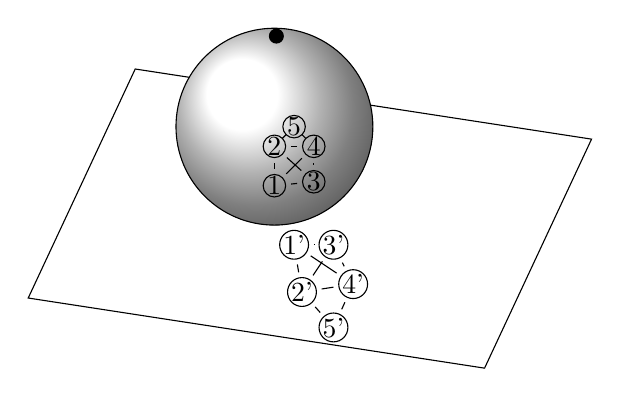
\begin{tikzpicture}[scale=0.5]
\tikzset{
 >=latex,
 inner sep=0pt,
outer sep=2pt,
mark coordinate/.style={inner sep=0pt,outer sep=0pt,minimum size=3pt,
    fill=black,circle}
}
\def\R{2.5} 
\def\angEl{35} 
\def\angAz{-105} 
\def\angPhi{-40} 
\def\angBeta{19} 

\pgfmathsetmacro\H{\R*cos(\angEl)}
\tikzset{xyplane/.style={cm={cos(\angAz),sin(\angAz)*sin(\angEl),-sin(\angAz),
                              cos(\angAz)*sin(\angEl),(0,-\H)}}}
\LongitudePlane[xzplane]{\angEl}{\angAz}
\LongitudePlane[pzplane]{\angEl}{\angPhi}
\LatitudePlane[equator]{\angEl}{0}


\draw[xyplane] (-2*\R,-2*\R) rectangle (2.2*\R,2.8*\R);
\filldraw[ball color=white] (0,0) circle (\R);
\foreach \t in {0} {\DrawLatitudeCircle[\R]{\t}}
\foreach \t in {80} { \DrawLongitudeCircle[\R]{\t} }


\node[circle,draw,minimum size=5pt,fill=black](0) at (0.05,2.3){};

%Der obere Graph:
\node[circle,draw](1) at (0,-1.5){1};
\node[circle,draw](2) at (0,-0.5){2};
\node[circle,draw](3) at (1,-1.4){3};
\node[circle,draw](4) at (1,-0.5){4};
\node[circle,draw](5) at (0.5,0){5};
\draw (1)--(2);
\draw (2)--(3);
\draw (3)--(4);
\draw (4)--(1);
\draw (1)--(3);
\draw (4)--(2);
\draw (4)--(5);
\draw (2)--(5);
%Der untere Graph:

\node[circle,draw](3') at (1.5,-3){3'};
\node[circle,draw](4') at (2,-4){4'};
\node[circle,draw](1') at (0.5,-3){1'};
\node[circle,draw](2') at (0.7,-4.2){2'};
\node[circle,draw](5') at (1.5,-5.1){5'};
\draw (1')--(2');
\draw (2')--(3');
\draw (3')--(4');
\draw (4')--(1');
\draw (1')--(3');
\draw (4')--(2');
\draw (4')--(5');
\draw (2')--(5');
\end{tikzpicture}
\caption{Stereographische Projektion}
\label{stP}
\end{figure}
Bisher haben wir Graphen noch nicht im dreidimensionalen Raum betrachtet. Könnte die räumliche Anordnung einen Unterschied in der überschneidungsfreien Einbettbarkeit von Graphen bewirken?  Betrachten wir zunächst einen $K_4$: Es wird deutlich, dass die Einbettung in eine Sphäre (z.\,B. die Erde) überschneidungsfrei möglich ist. Unterscheidet sich dieser dann aber von einem $K_4$, der in eine Ebene eingebettet wurde? Geometrisch gesehen wäre das eindeutig der Fall -- in dem von uns betrachteten Gebiet, der Graphentheorie, jedoch nicht, da über seine \wichtig{stereographische Projektion} auf eine Ebene der Graph weiterhin planar abgebildet würde.
Diese Projektion, wie sie in Abbildung \ref{stP} zu sehen ist, lässt sich wie folgt veranschaulichen: Eine Lampe, die sich im \glqq Nordpol\grqq\ der Sphäre befindet, wirft von innen heraus einen Schatten des Graphen auf die Ebene. Ein typisches Anwendungsbeispiel für diese Projektion ist die Kartografie. 



%\begin{figure}
%\begin{tikzpicture}[scale=0.5]
%\node(1) at (0,0){};
%\node(2) at (0,2){};
%\node(3) at (0,2.5){};
%\node(4) at (0,4){};
%\node(5) at (3,4){};
%\node(6) at (3,2.5){};
%\node(7) at (3,2){};
%\node(8) at (3,0){};
%\node(9) at (1.5,4){};
%\node(10) at (1.5,0){};

%\draw[->] (1) to (2);
%\draw[->] (2) to (3);
%\draw[->] (4) to (9);
%\draw[->] (8) to (7);
%\draw[->] (7) to (6);
%\draw[->] (1) to (10);

%\draw (0,0) rectangle (3,4);
%\end{tikzpicture}

%\begin{tikzpicture}[scale=0.5]
%\draw(0,0) ellipse (1cm and 0.5cm);
%\draw (1,0)--(1,-4);
%\draw(-1,0)--(-1,-4);
%\draw(1,-4) arc (0:-180:1 and 0.5); 
%\node(1) at (-0.1,-0.50){};
%\node(2) at (0.1,-0.5){};
%\draw[->](2) to (1);
%\node(1) at (-0.1,-4.50){};
%\node(2) at (0.1,-4.5){};
%\draw[->](2) to (1);
%\end{tikzpicture}

%\begin{tikzpicture}[scale=0.5]
  %\draw (-1,0) to[bend left] (1,0);
  %\draw (-1.2,.1) to[bend right] (1.2,.1);
  %\draw[rotate=0] (0,0) ellipse (100pt and 50pt);
%\end{tikzpicture}
%\caption{Quadrat zu Torus}
%\label{Q2T}
%\end{figure}

\begin{figure}
	\centering
		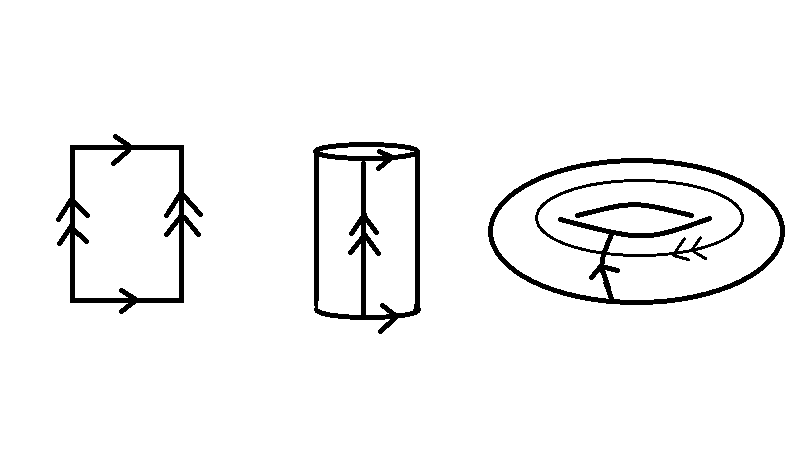
\includegraphics[width=7cm]{img/2to3D.png}
\caption{Vom Rechteck zum Torus}
\label{Q2T}
\end{figure}

Da die Einbettung in die Sphäre keinen Unterschied zur Ebene bezüglich der überschneidungsfreien Einbettbarkeit eines Graphen macht, betrachten wir nun ein weiteres topologisches Gebilde: einen \wichtig{Torus} (vergleichbar mit einem Donut). Sowohl Torus als auch Sphäre bezeichnet man als sogenannte \wichtig{kompakte, orientierbare Mannigfaltigkeiten}, die sich durch die Anzahl ihrer Löcher charakterisieren. Bei einer Sphäre sind dies null, beim Torus eins, beim Doppeltorus zwei, usw. Demnach sind mathematisch betrachtet also auch ein Donut und eine Kaffetasse gleiche räumliche Gebilde.
Um die Darstellung eines Graphen z.\,B. auf einem Torus oder einer Sphäre zu vereinfachen, verwendet man \wichtig{Verklebungen}, eine zweidimensionale Abbildungsmöglichkeit, bei der Schnittkanten den dreidimensionalen Körper zu einer Fläche aufklappbar machen. Das schrittweise Verkleben dieser Schnittkanten von Rechteck zu Torus wird in Abbildung \ref{Q2T} veranschaulicht.

\begin{figure}
	\centering
		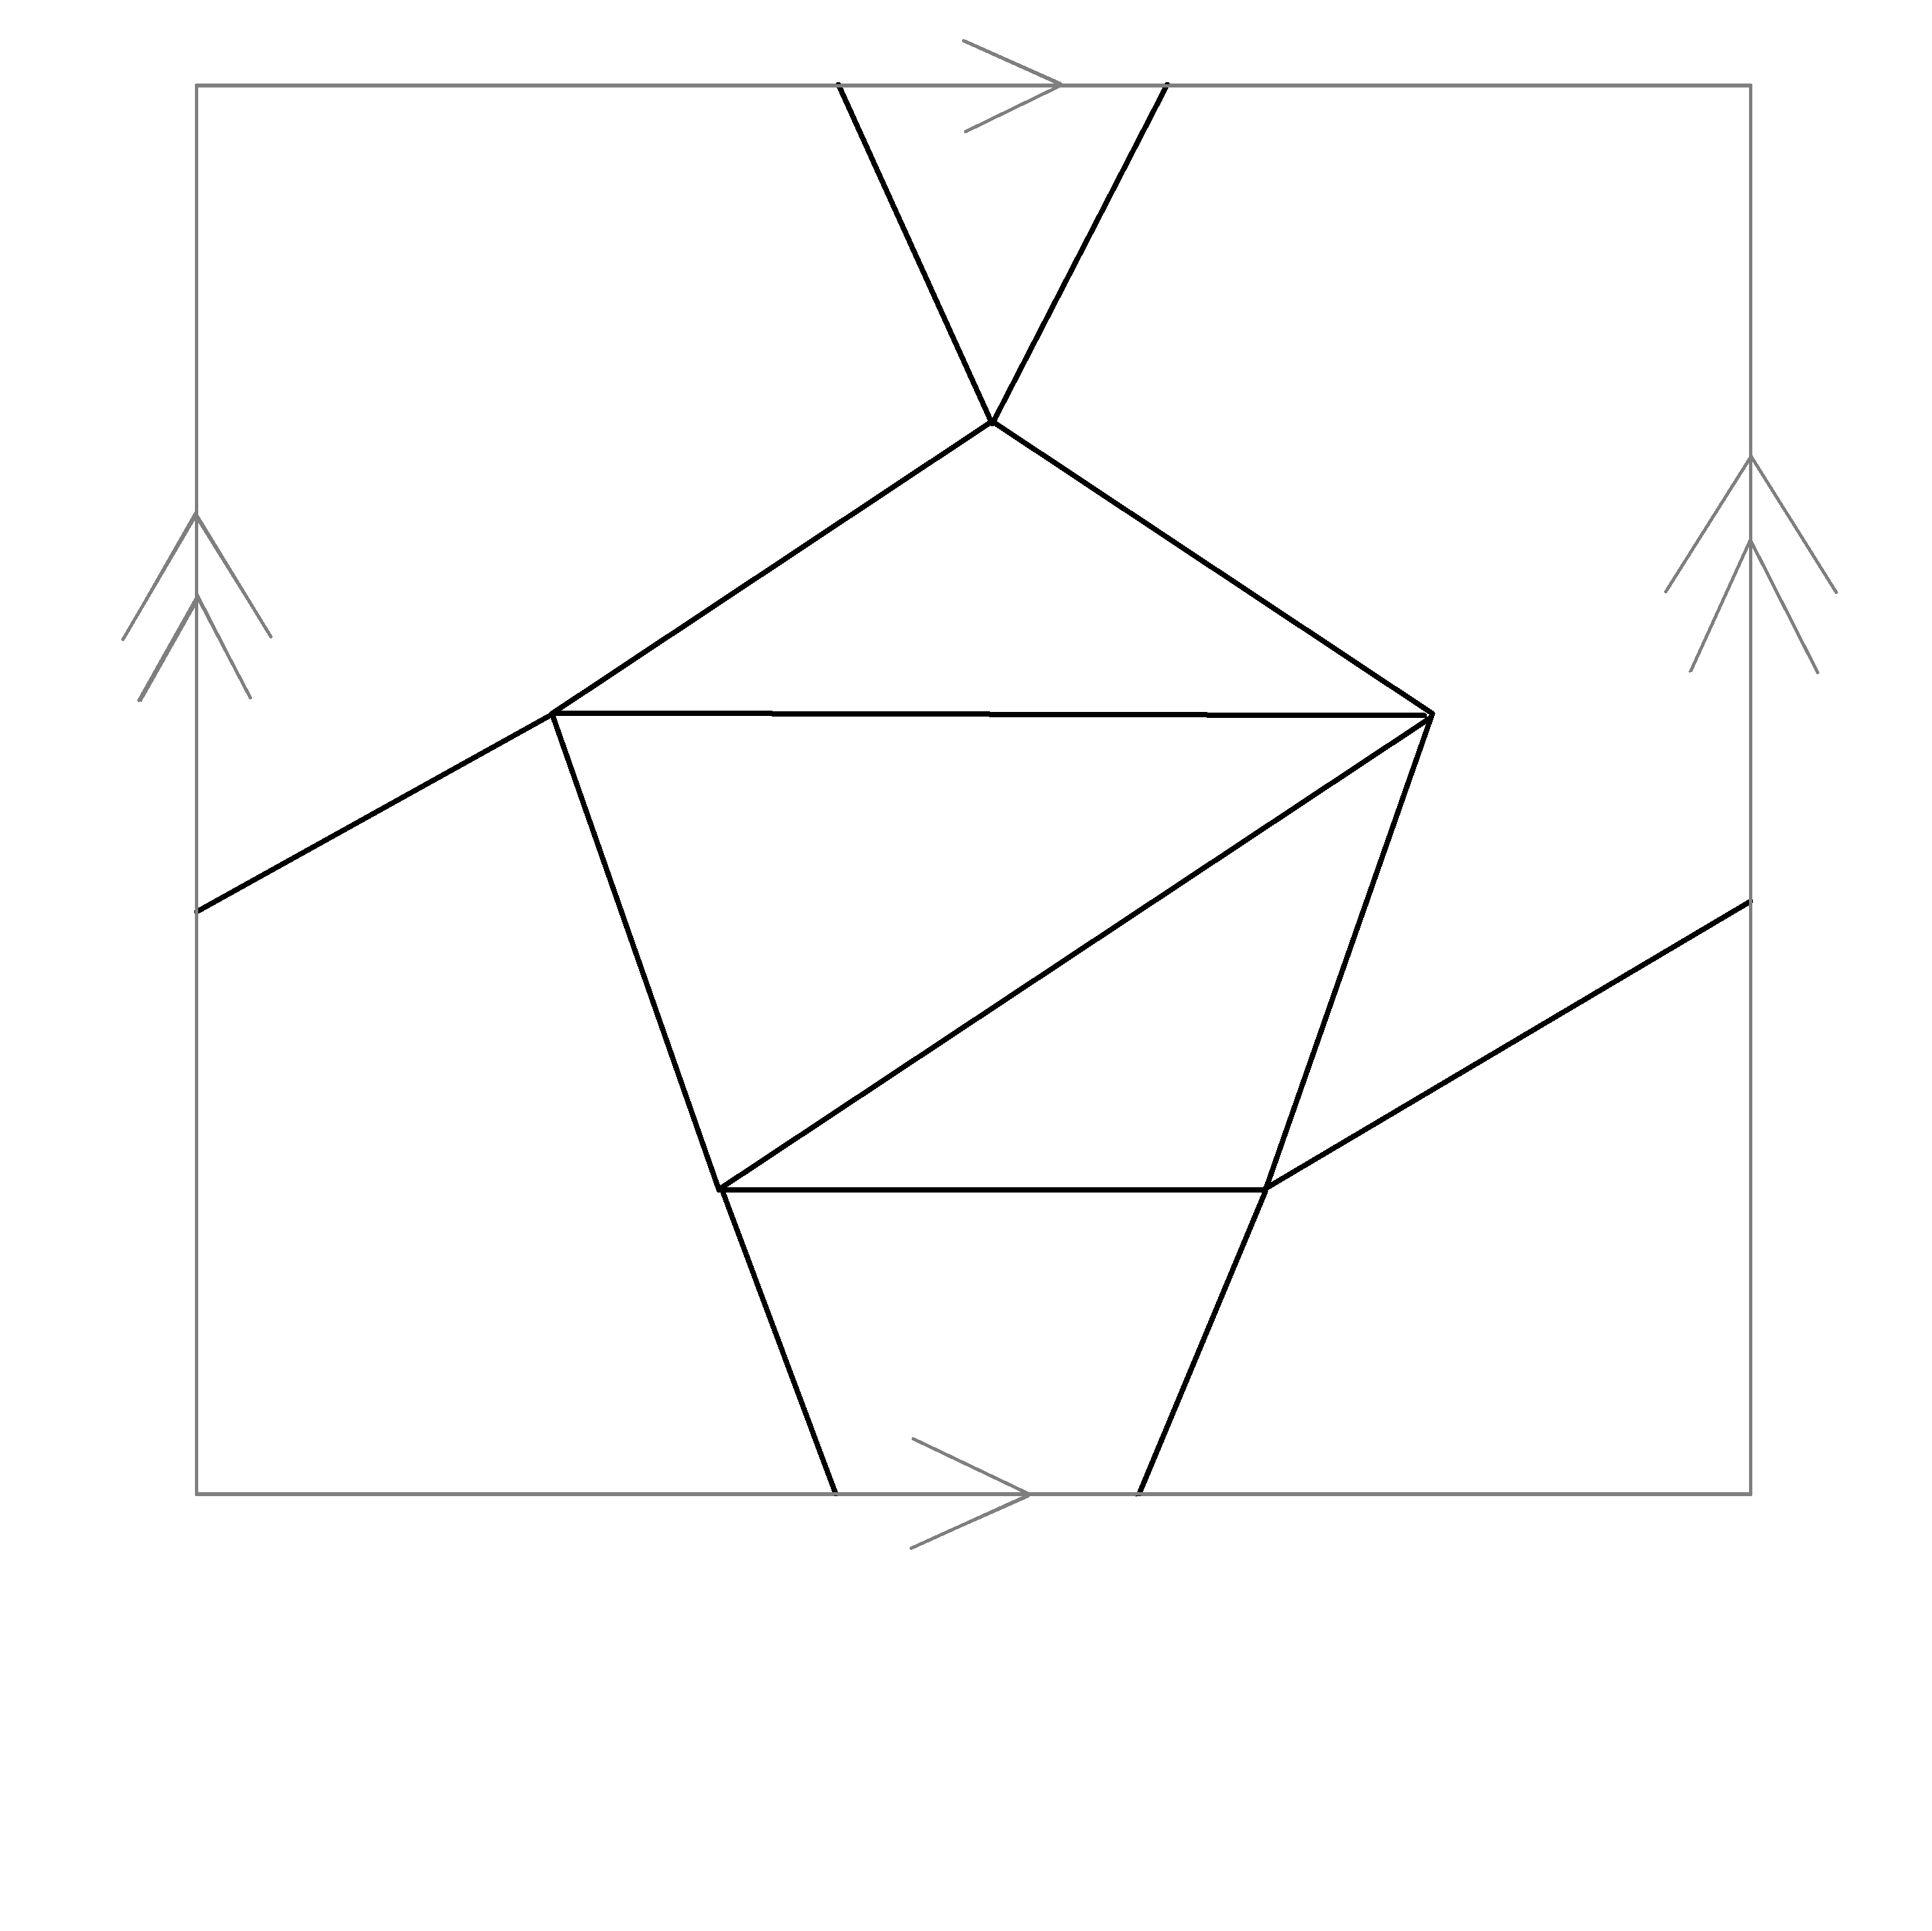
\includegraphics[width=7cm]{img/K5.png}
\caption{$K_5$}
\label{k5}
\end{figure}
Aus dem Satz von Kuratowski leitet sich nun folgende Fragestellung ab: Welche $K_{n}$ sind auf dem Torus überschneidungsfrei einbettbar? Im Folgenden betrachten wir insbesondere den $K_5$ als nicht-planaren, vollständigen Graphen auf dem Torus noch einmal genauer.
Hierfür bilden wir zunächst den Graphen zweidimensional ab und springen dabei für die Kanten -- falls notwendig -- an den Schnittkanten der Verklebung zur gegenüberliegenden Seite, wie in Abbildung \ref{k5}  zu sehen ist. Der $K_5$ ist nach dieser Vorgehensweise auf dem Torus überschneidungsfrei einbettbar und es wird somit deutlich, dass für die überschneidungsfreie Einbettung auf einem Torus der Satz von Kuratowski nicht gilt.

Allgemein ist bekannt, dass sich bei $\lceil \frac{(n-3)(n-4)}{12} \rceil$ Löchern einer Mannigfaltigkeit entsprechend der $K_{n}$ überschneidungsfrei einbetten lässt. Von $n = 5$ bis einschließlich $n = 7$ liefert diese Formel $1$ als Lösung, weshalb für den Torus der $K_7$ der maximale vollständige Graph ist, der sich überschneidungsfrei einbetten lässt.

